% ------------------------------------------------------------------------
% file `main-bookexercise-7-exercise-body.tex'
%
%     exercise of type `bookexercise' with id `7'
%
% generated by the `exercise' environment of the
%   `xsim' package v0.21 (2022/02/12)
% from source `main' on 2026/10/27 on line 2247
% ------------------------------------------------------------------------
1. （某年408真题）使用迪杰斯特拉算法求下图中顶点1到其他各顶点之间的最短路径，则依次确定最短路径的目标定点是\underline{\hspace{1cm}}
\begin{center}
    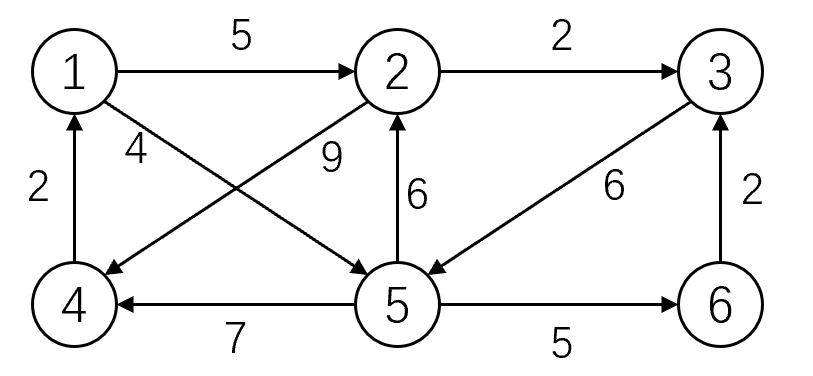
\includegraphics[width=0.40\textwidth]{assets/pics_and_ppts/ch5/习题09，16408最短路径的选点顺序.png}
\end{center}

\begin{tabular}{llll}
    A. 5,2,3,4,6 & B. 5,2,3,6,4 & C. 5,2,4,3,6 & D. 5,2,6,3,4
\end{tabular}

\vspace{\baselineskip}

2. （某年408真题）对下图所示的有向带权图，若采用迪杰斯特拉算法求源点a到其他各顶点的最短路径，则第一个确定全局最短路径的顶点是b，第二个确定全局最短路径
的顶点是c，后续的顶点依次是\underline{\hspace{1cm}}

\begin{center}
    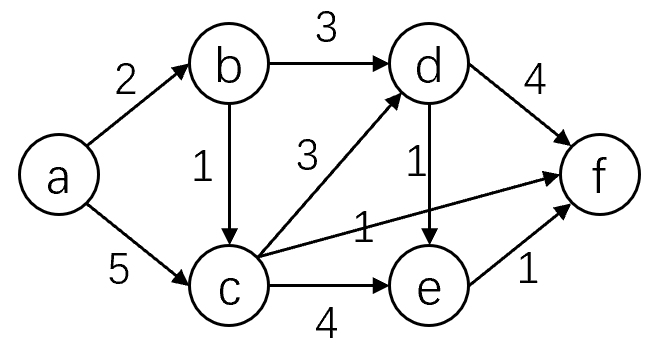
\includegraphics[width=0.34\textwidth]{assets/pics_and_ppts/ch5/习题10，12408最短路径选点顺序.png}
\end{center}

\begin{tabular}{llll}
    A. d,e,f & B. e,d,f & C. f,d,e & D. f,e,d
\end{tabular}

\vspace{\baselineskip}

3. （某年408真题）使用迪杰斯特拉算法求下图中从顶点1到其余各顶点的最短路径，将当前找到的从顶点1到顶点2，3，4，5的最短路径
保存在数组dist[]中，则依次求出两个顶点（不包括源点1）的最短路径后，dist中的内容更新为\underline{\hspace{1cm}}

\begin{center}
    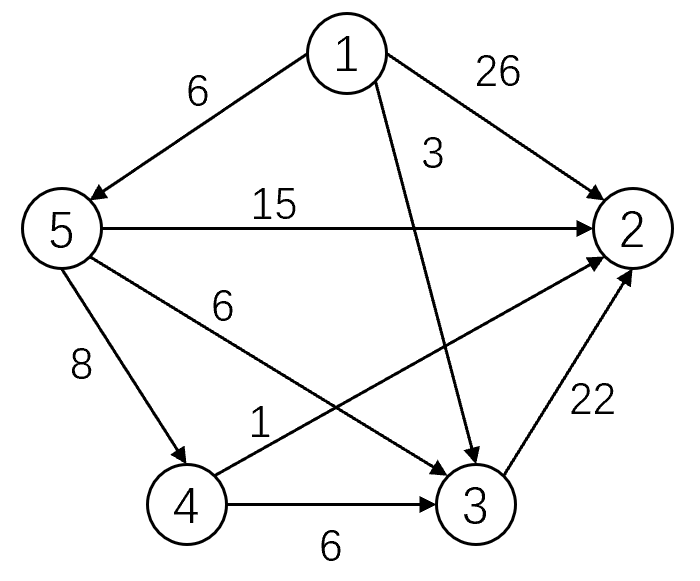
\includegraphics[width=0.33\textwidth]{assets/pics_and_ppts/ch5/习题11，21408迪杰斯特拉dist内容.png}
\end{center}

\begin{tabular}{llll}
    A. 26,3,14,6 & B. 25,3,14,6 & C. 21,3,14,6 & D. 15,3,14,6
\end{tabular}

\vspace{\baselineskip}

4. 请你说明：迪杰斯特拉算法、Bellman-Ford算法以及SPFA算法应对以下情况的图时会怎样？\\[0.5em]
a）存在从源点可达的负环；\\
b）不存在从源点可达的负环，但存在从源点可达的负权边；\\

维火女被邪恶的恶魔、大陆守护神的孪生兄弟LoopCore抓了起来，并关在了监牢的某个牢房里。监牢可以被建模为一个图$G=(V,E)$，顶点表示牢房。

已知该监牢有 $N$ 个牢房，编号为 0 到 $N-1$，牢房之间均存在双向通路，用邻接表存储图模型。你毫不犹豫地动身前往牢房营救维火女，但你破门而入后意外地被魔法传送进了牢房s。\\

5. 已知每个牢房（顶点）的数据类型为char：维火女所在的牢房为\textquotesingle T\textquotesingle，其余牢房均为\textquotesingle F\textquotesingle。
给出在每两个牢房之间移动所需要花费的时间time\_cost（非负），请你计算从s出发，到达维火女的房间所需要的最短时间是多少，若无法到达，返回-1。

\begin{cppcode}
    // N 已定义
    struct EdgeInfo {
        int u;          // 顶点编号
        int time_cost;  // 花费时间（边权）
    };
    vector<EdgeInfo> AdjList[N];    // 已存储邻接表信息
    char ver_info[N];   // 已存储顶点信息
    // 返回以s为起点到达维火女的房间需要花费的最短时间
    int MinTime(int s) {

    }
\end{cppcode}

\vspace{\baselineskip}

6. 在{\color{red}上题}条件下，假设你在任何两个房间移动时需要和敌人战斗，此时边（Edge）使用如下结构定义：
\begin{cppcode}
    struct EdgeInfo {
        int u;
        int time_cost;      // 花费时间
        int energy_cost;    // 和敌人战斗需要消耗的能量值
    };
\end{cppcode}
保证所有边的time\_cost和energy\_cost均非负。你决定选择所有路线中，消耗时间最少的路线去营救维火女。若有多条路线消耗时间相等，你将选择其中
消耗能量最少的一条路线。

编写一个函数，返回你所选择的路线所消耗的能量值。若无法到达，返回-1。\\

% *7. 在{\color{red}上题}条件下，若你的初始能量值为$e_1$，并且在你到达维火女的房间后，至少还剩有$e_2$的能量值的前提下，才能带她一起离开监牢。
% 现要求你找到她后，必须能够带她离开监牢。在此前提下，你将选择时间最短的一条路线，若有多条路线，你将选择消耗能量最少的路线。请返回在此路线下你
% 到达维火女的房间时剩余的能量值。

% \begin{cppcode}
%     // N 已定义
%     struct EdgeInfo {
%         int u;
%         int time_cost;      // 花费时间
%         int energy_cost;    // 和敌人战斗需要消耗的能量值
%     };
%     vector<EdgeInfo> AdjList[N];    // 已存储邻接表信息
%     char ver_info[N];   // 已存储顶点信息
%     // 返回以s为起点到达维火女的房间需要花费的最短时间
%     int RemainingEnergy(int s, int e1, int e2) {

%     }
% \end{cppcode}



